% fig9-state-machines.tex — Figure 9: State transitions (DEV-GOV-03)
%
% Three machines that are routinely read as one. They are drawn separately on
% purpose: the whole class of "zero findings looked like a pass" bugs comes from
% collapsing the middle column into the right one.
%
% Every label here is a real serialised value: ReviewParseStatus,
% ReviewFindingStatus and ReviewCardConfidence in runtime/src/code_review/report.rs
% and rusty-claude-cli/src/review_card.rs.
%
% Layout notes: every state box has a fixed text width, so the spacing between
% columns is predictable. Letting the boxes size to their text put
% `parse_attempted_but_failed` on top of its neighbour.
\documentclass[tikz,border=10pt]{standalone}
\usetikzlibrary{arrows.meta,positioning,fit,backgrounds,calc}

\begin{document}
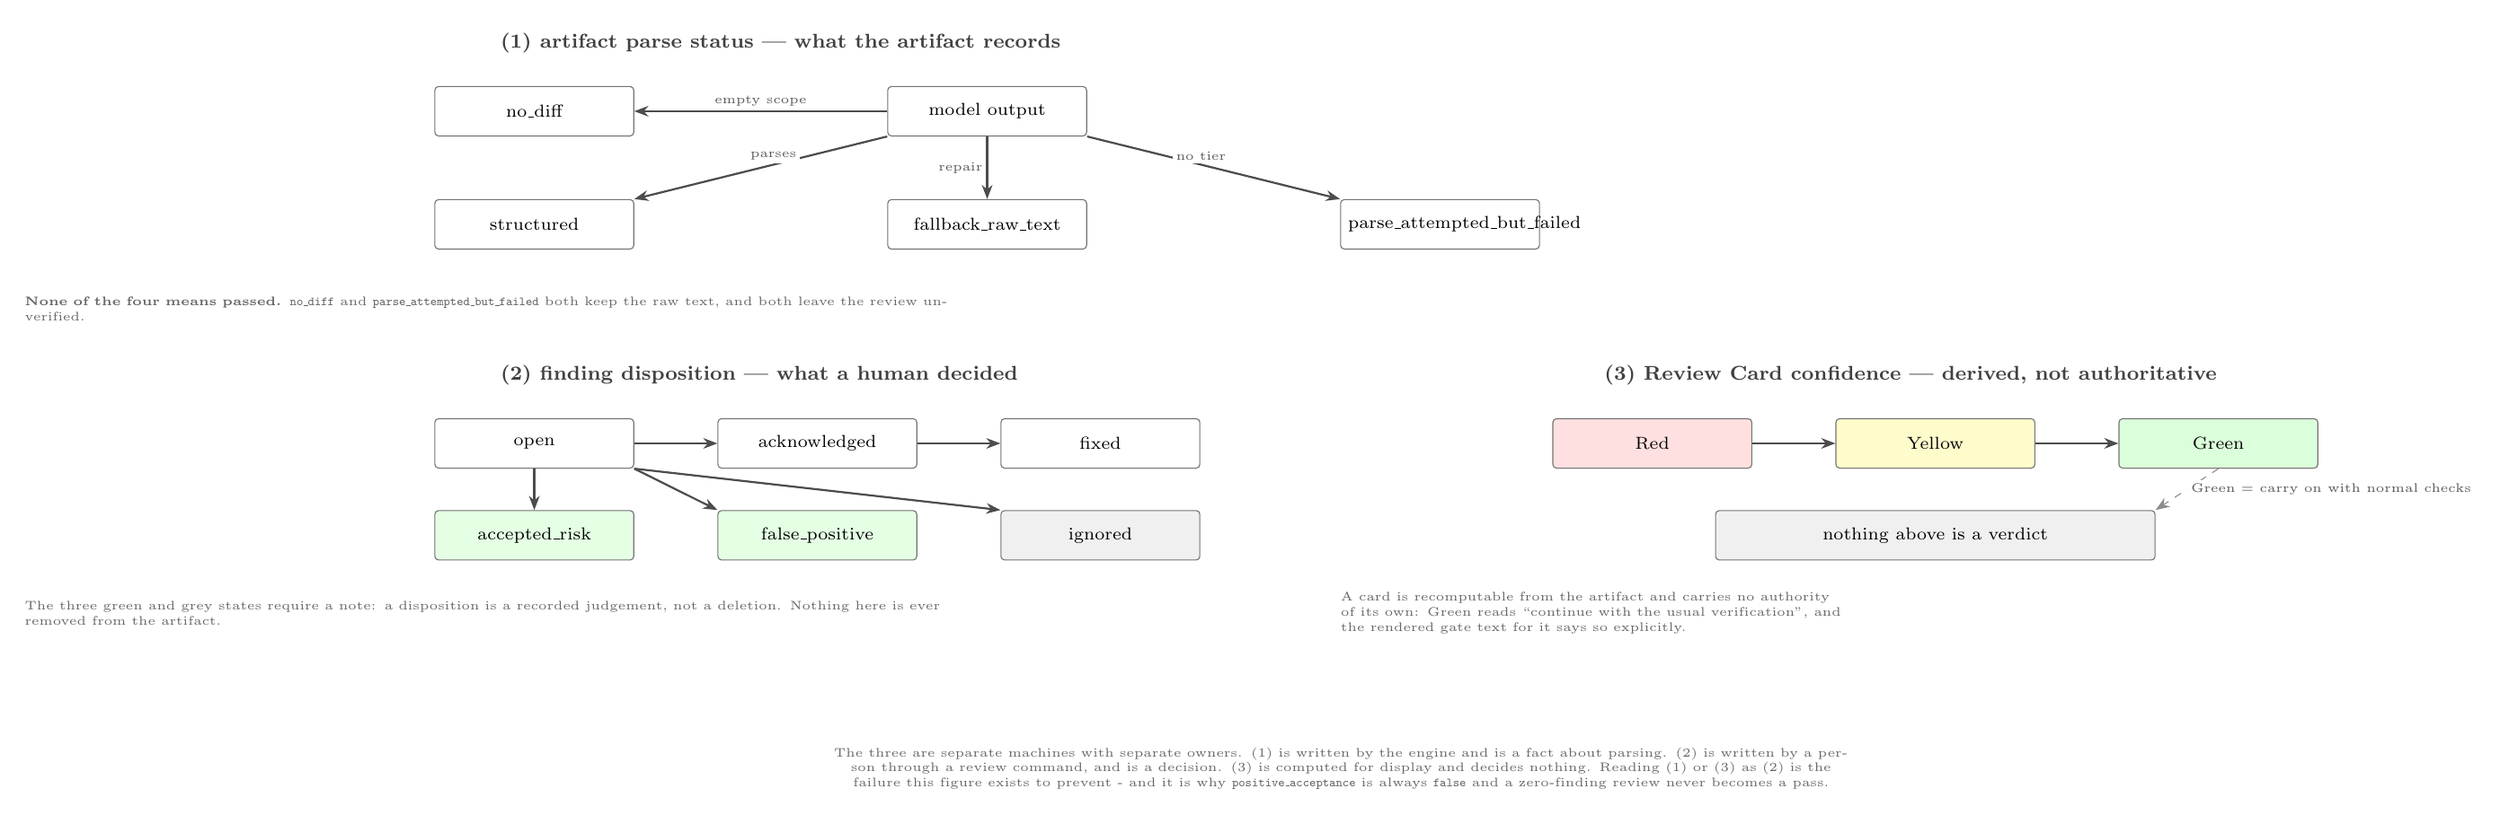
\begin{tikzpicture}[
  x=1cm, y=1cm,
  font=\small,
  st/.style={draw, rounded corners=1.5pt, fill=white, draw=black!55,
             font=\scriptsize, align=center, inner sep=3pt,
             text width=26mm, minimum height=7mm},
  term/.style={st, fill=black!6},
  arr/.style={-{Stealth[length=2mm]}, thick, draw=black!70},
  arrd/.style={-{Stealth[length=2mm]}, draw=black!45, dashed},
  lab/.style={font=\tiny, text=black!65, inner sep=1.5pt, fill=white},
  note/.style={font=\tiny, text=black!60, align=left, inner sep=0pt},
  title/.style={font=\footnotesize\bfseries, text=black!75, anchor=south west}
]

% ================= (1) parse status =================
\node[title] at (-14.0, 7.0) {(1) artifact parse status --- what the artifact records};
\node[st] (in) at (-7.0, 6.3) {model output};
\node[st] (nodiff) at (-13.4, 6.3) {no\_diff};
\node[st] (struct) at (-13.4, 4.7) {structured};
\node[st] (fb) at (-7.0, 4.7) {fallback\_raw\_text};
\node[st] (pf2) at (-0.6, 4.7) {parse\_attempted\_but\_failed};

\draw[arr] (in.west) -- node[lab, above] {empty scope} (nodiff.east);
% From the source box, not from `in.west |- struct`: that coordinate sits on the
% right edge of the fallback box, so the edge looked like it started there.
\draw[arr] (in.south west) -- node[lab, above, pos=0.45] {parses} (struct.north east);
\draw[arr] (in.south) -- node[lab, left] {repair} (fb.north);
\draw[arr] (in.south east) -- node[lab, above, pos=0.45] {no tier} (pf2.north west);

\node[note, text width=132mm] at (-14.0, 3.5)
  {\textbf{None of the four means passed.} \texttt{no\_diff} and \texttt{parse\_attempted\_but\_failed} both keep the raw
   text, and both leave the review unverified.};

% ================= (2) finding disposition =================
\node[title] at (-14.0, 2.3) {(2) finding disposition --- what a human decided};
\node[st] (open) at (-13.4, 1.6) {open};
\node[st] (ack) at (-9.4, 1.6) {acknowledged};
\node[st] (fixed) at (-5.4, 1.6) {fixed};
\node[st, fill=green!10] (ar) at (-13.4, 0.3) {accepted\_risk};
\node[st, fill=green!10] (fp) at (-9.4, 0.3) {false\_positive};
\node[term] (ig) at (-5.4, 0.3) {ignored};
\draw[arr] (open.east) -- (ack.west);
\draw[arr] (ack.east) -- (fixed.west);
\draw[arr] (open.south) -- (ar.north);
\draw[arr] (open.south east) -- (fp.north west);
\draw[arr] (open.south east) -- (ig.north west);

\node[note, text width=132mm] at (-14.0, -0.8)
  {The three green and grey states require a note: a disposition is a recorded judgement, not a deletion. Nothing here is ever
   removed from the artifact.};

% ================= (3) review card =================
\node[title] at (1.6, 2.3) {(3) Review Card confidence --- derived, not authoritative};
\node[st, fill=red!12] (red) at (2.4, 1.6) {Red};
\node[st, fill=yellow!20] (yel) at (6.4, 1.6) {Yellow};
\node[st, fill=green!14] (grn) at (10.4, 1.6) {Green};
\draw[arr] (red.east) -- (yel.west);
\draw[arr] (yel.east) -- (grn.west);

\node[term, text width=60mm] (only) at (6.4, 0.3) {nothing above is a verdict};
\draw[arrd] (grn.south) -- node[lab, right] {Green = carry on with normal checks} (only.north east);

\node[note, text width=72mm] at (1.6, -0.8)
  {A card is recomputable from the artifact and carries no authority of its own: Green reads ``continue with the usual
   verification'', and the rendered gate text for it says so explicitly.};

% ================= the boundary =================
\node[note, text width=184mm, align=center] at (-2.0, -3.0)
  {The three are separate machines with separate owners. (1) is written by the engine and is a fact about parsing. (2) is
   written by a person through a review command, and is a decision. (3) is computed for display and decides nothing. Reading
   (1) or (3) as (2) is the failure this figure exists to prevent - and it is why \texttt{positive\_acceptance} is always
   \texttt{false} and a zero-finding review never becomes a pass.};

\end{tikzpicture}
\end{document}
